\chapter{Wykorzystane narzędzia}
Podczas realizacji tematu pracy wykorzystanych zostało wiele narzędzi rozumianych jako języki programowania, biblioteki, środowiska programistyczne, czy inne technologie. W niniejszym rozdziale przedstawione i dokładniej opisane zostały te, które odegrały kluczową rolę.

\section{Język Python}
Python\furl{https://python.org} jest jednym z najpopularniejszych języków wykorzystywanych do analizy danych oraz uczenia maszynowego. Jest zresztą ogólnie jednym z najpopularniejszych języków, co zostało potwierdzone przez badanie \bibtitle{2023 Developer Survey} \mycite{stackoverflow-survey}, gdzie uplasował się na 4. miejscu w rankingu popularności.

Python wykorzystano ze względu na ogromną liczbę bibliotek, które są dla niego dostępne. Kilka spośród nich, które odegrały kluczową rolę podczas realizacji niniejszego tematu, zostało opisanych w poniższych sekcjach. Ponadto umożliwia on bardzo szybkie prototypowanie i eksperymentowanie, co również zostało docenione. Jest to bowiem język wysokopoziomowy i zwalnia programistów z zajmowania się wieloma kwestiami. Jest elastyczny ze względu na swoje wieloparadygmatowe podejście: obiektowe, proceduralne, jak i funkcyjne. Ostatecznie jest językiem skryptowym i brak narzutu czasowego na kompilację znacznie skraca pętlę zwrotną między pisaniem kodu a obserwowaniem jego skutków.

\subsection{Biblioteka PyTorch}
Biblioteka \code{PyTorch}\furl{https://pytorch.org} stanowi potężne narzędzie w obszarze uczenia maszynowego i głębokiego uczenia. Pozwala na tworzenie i szkolenie różnorodnych modeli sieci neuronowych, a charakteryzuje się przy tym elastycznością i wydajnością.  Jej moduły obejmują wsparcie dla operacji tensorowych, automatyczne różniczkowanie (co ułatwia proces uczenia się sieci), a także obsługę zarówno CPU, jak i GPU do przyspieszenia obliczeń. Jednym z największych atutów biblioteki \code{PyTorch} jest prostota w tworzeniu modeli. Dzięki intuicyjnej składni oraz dynamicznemu grafowi obliczeniowemu użytkownicy mogą szybko prototypować, testować i dostosowywać swoje modele, co sprawia, że jest szczególnie popularnym wyborem dla zastosowań badawczych.

\subsection{Biblioteki SpaCy i Stanza}
Biblioteki \code{SpaCy}\furl{https://spacy.io} i \code{Stanza}\footnote{\url{https://stanfordnlp.github.io/stanza}} to popularne dla języka Python drogi do przeprowadzenia analizy tekstów w języku naturalnym. Zostały przedstawione razem, ponieważ różnice między nimi są niewielkie i za pomocą obu można realizować niemal identyczne cele. O wykorzystaniu pierwszej lub drugiej zadecydowały mało istotne szczegóły, takie jak interfejs, który w danym momencie wydawał się wygodniejszy. Z powodzeniem można by było jednak ograniczyć się do wykorzystania jednej z nich.

Obie z przytoczonych bibliotek pozwalają na analizę tekstów w różnych językach, w tym języku polskim. Pozwalają na przeprowadzenie tokenizacji, czyli podziału tekstów na poszczególne słowa oraz lematyzacji, czyli zamiany każdego słowa na jego bazową formę. Można za ich pomocą znaleźć w tekście wszystkie nazwy własne poprzez analizę \code{NER} \mycite{liu2022overview}, czy też przypisać do każdego słowa nazwę części mowy, którą stanowi. 

\subsection{Biblioteka SQLParse}
Biblioteka \code{SQLParse}\furl{https://sqlparse.readthedocs.io} nie jest wyjątkowo rozbudowana pod względem oferowanych funkcji, lecz jej niezaprzeczalna popularność sugeruje, że doskonale wpasowała się w potrzeby deweloperów. Tak jak mówi nazwa, \code{SQLParse} pozwala na parsowanie zapytań SQL. Sprowadza się to do konwersji podanego jako wejście zapytania na poszczególne tokeny, takie jak słowa kluczowe \code{SELECT}, \code{WHERE}, nazwy kolumn i tabel oraz wartości. Każdy z wyprodukowanych przy tym tokenów posiada typ, mówiący co sobą reprezentuje. Biblioteka ta odegrała istotną rolę w procesie przygotowywania polskich zbiorów danych.

\subsection{Biblioteka SQLGlot}
Biblioteka \code{SQLGlot}\furl{https://sqlglot.com} to naprawdę rozbudowane i wszechstronne narzędzie służące do pracy z instrukcjami SQL. Wspiera ponad 20 różnych dialektów i pozwala na transpilację, czyli konwersję instrukcji SQL pomiędzy nimi. Ponadto zapewnia szczegółową walidację i formatowanie. Wśród jej bardziej zaawansowanych funkcji znajduje się optymalizacja zapytań, a nawet symulowanie całego silnika bazodanowego, co pozwala na wykonywanie przez nią instrukcji.

Najbardziej pożądaną podczas realizacji niniejszej pracy funkcją okazało się parsowanie zapytań do drzew \code{AST} (ang. Abstract Syntax Tree) oraz możliwość dalszej pracy z nimi. Są to struktury, które pozwalają na reprezentację programów, czy też instrukcji w dowolnym języku formalnym, w wygodnej do analizy i modyfikacji postaci. Drzewo \code{AST} dla przykładowego zapytania SQL zostało przedstawione na rysunku \ref{fig:sql-ast-example}.

\begin{figure}[ht!]
  \centering
  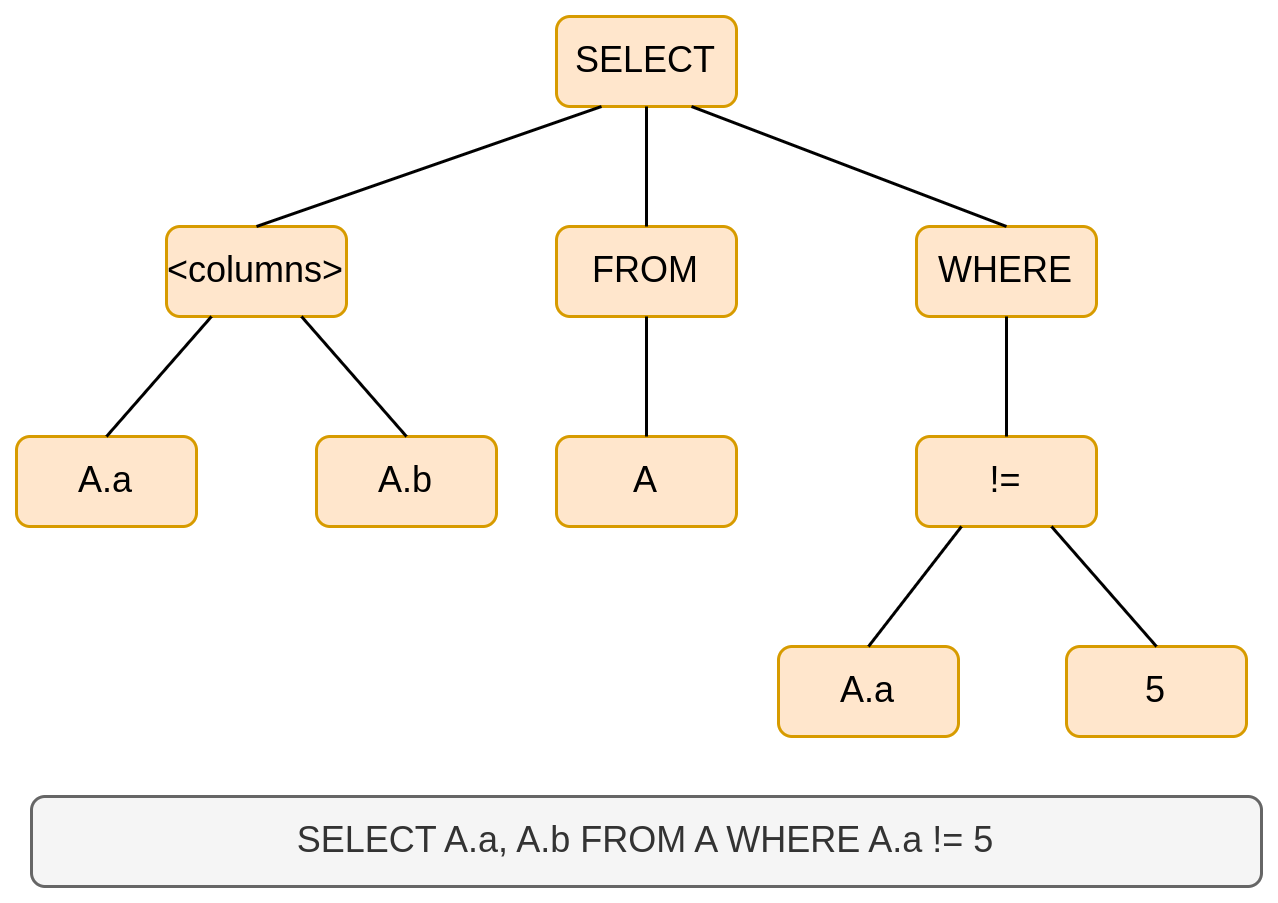
\includegraphics[width=0.55\linewidth]{images/ast_example.png}
  \caption{Drzewo \code{AST} dla przykładowego zapytania SQL}
  \label{fig:sql-ast-example}
\end{figure}

\subsection{Biblioteka Streamlit}
Biblioteka \code{Streamlit}\furl{https://streamlit.io} stanowi narzędzie do szybkiego tworzenia interaktywnych aplikacji internetowych opartych na danych. Została zaprojektowana z myślą o prostocie użycia, umożliwiając nawet początkującym programistom szybkie tworzenie interfejsów graficznych, bez konieczności dużej wiedzy na temat frontendu. 

\code{Streamlit} oferuje intuicyjną składnię, która umożliwia tworzenie aplikacji poprzez strumieniowe przetwarzanie danych. Zapewnia integrację z wieloma bibliotekami do analizy danych i uczenia maszynowego. Jedną z kluczowych cech \code{Streamlit} jest automatyczne odświeżanie interfejsu użytkownika w odpowiedzi na zmiany w kodzie, co pozwala na szybką iterację i testowanie aplikacji. Dodatkowo biblioteka oferuje szeroki zakres interaktywnych elementów interfejsu, takich jak suwaki, pola wyboru, czy wykresy, które mogą być łatwo integrowane z analizowanymi danymi. W kontekście niniejszej pracy magisterskiej biblioteka \code{Streamlit} została wykorzystana w celu stworzenia aplikacji pozwalającej na praktyczne wykorzystanie opracowanych rozwiązań.

\section{Visual Studio Code}
Visual Studio Code\furl{https://code.visualstudio.com} to wszechstronny edytor stworzony przez Microsoft. Zgodnie z wcześniej wspomnianą ankietą \bibtitle{2023 Developer Survey} \mycite{stackoverflow-survey} jest on najczęściej wybieranym przez deweloperów środowiskiem programistycznym. Tym, co je wyróżnia, jest prostota przy jednoczesnej potędze płynącej z niespotykanej elastyczności. Dostępna jest bowiem ogromna liczba łatwych w instalacji rozszerzeń. Pozwalają one dostosować to środowisko niemal do każdego scenariusza wykorzystania.

Podczas realizacji pracy szczególnie użyteczne okazały się rozszerzenia dla języka Python dodające kolorowanie składni, dokończanie kodu, debugowanie, czy też wsparcie dla interaktywnych notesów \code{Jupyter}. Poza tym intensywnie wykorzystywane było rozszerzenie do pracy z narzędziem \code{Docker}. Jeśli chodzi o podstawowe funkcje środowiska, to bardzo użyteczna okazała się integracja z systemem kontroli wersji oraz zaawansowane wyszukiwanie i zastępowanie.

\section{Docker}
\code{Docker}\furl{https://www.docker.com} to bardzo potężne i powszechnie wykorzystywane narzędzie, na którym opiera się znaczna część funkcjonującego oprogramowania. Umożliwia on tworzenie, zarządzanie i uruchamianie aplikacji w niemal całkowicie izolowanych środowiskach zwanych kontenerach. Pozwalają one deweloperom na zapakowanie aplikacji z zależnościami i środowiskiem uruchomieniowym, co zapewnia spójność działania na różnych platformach.

Podczas realizacji niniejszego projektu \code{Docker} okazał się szczególnie użyteczny w kontekście uruchamiania istniejących modeli uczenia maszynowego. Część z nich była od razu gotowa do działania w kontenerze, a inne zostały do tego przystosowane. Okres czasu, w którym analizowane w dalszej części pracy rozwiązania powstawały jest bowiem bardzo rozległy, więc zależności z których korzystają znacznie się różnią i trudno jest je ze sobą pogodzić. W przypadku prostych różnic w pakietach języka Python możliwe jest skorzystanie ze znacznie prostszego narzędzia \code{Conda}, lecz poziom izolacji tworzonych za jego pomocą środowisk jest znacznie ograniczony i jak się okazało często niewystarczający.

\section{Platforma Hugging Face}
\code{Hugging Face}\furl{https://huggingface.co} to platforma dostarczająca narzędzia do tworzenia rozwiązań uczenia maszynowego. Zgromadzona jest na niej ogromna liczba pretrenowanych modeli i zbiorów danych, które może dodawać każdy. Dzięki temu zyskała ogromną popularność wśród projektów \code{open source} oraz badaczy. Nie jest to jednak wyłącznie platforma, ale także liczna społeczność, której celem jest zapewnienie równego dostępu do rozwiązań sztucznej inteligencji.

Korzystanie z zasobów udostępnionych przez \code{Hugging Face} jest niezwykle proste. Po wyszukaniu odpowiedniego modelu lub zbioru w interfejsie graficznym, wystarczy zwykle skopiować jego identyfikator i dodać do swojego skryptu jedną lub kilka linijek kodu. \code{HF} w szczególności skupia się na przetwarzaniu języka naturalnego i dostarcza do języka Python bibliotekę \code{transformers}. Daje ona możliwość konfigurowania, uruchamiania i trenowania modeli bazujących na architekturze transformerów \mycite{NIPS2017_3f5ee243}, która daje obecnie najlepsze wyniki, jeśli chodzi właśnie o język naturalny. 
